\pdfminorversion=7

\documentclass{beamer}
\beamertemplatenavigationsymbolsempty
\usetheme{Boadilla}

\usepackage[utf8]{inputenc}
\usepackage[english]{babel}
\usepackage{graphicx}
\usepackage{tikz}
\usepackage{booktabs}
\usepackage{siunitx}
\usepackage{amsmath}
\usepackage{verbatim}
\usetikzlibrary{automata, positioning, arrows}
\usepackage{xcolor}
\usepackage{hyperref}
\usepackage{tabularx}
\usepackage{booktabs}
\usepackage{natbib}

\usepackage{colortbl}
\usepackage{textcomp}
\usepackage{amssymb}
\usepackage{amsthm} % theorems and lemmas
\usepackage{mathpartir} % type inference rules
\usepackage{lineno} % line numbers (good for reviewing)
\usepackage{stmaryrd} % double square brackets
\usepackage{mathtools}
\usepackage{listings}
\usepackage{wrapfig}

% Define Lua blue
\definecolor{LuaBlue}{RGB}{0, 0, 128}

% Apply Lua blue to beamer structure
\setbeamercolor{structure}{fg=LuaBlue}

% % Uncomment the following lines for the production version
% \setbeamertemplate{frametitle continuation}{\insertcontinuationcount}
% \beamerdefaultoverlayspecification{<+->}

\usetikzlibrary{positioning}

\tikzset{
    wf/.style={temporal={#1{}{color=orange}{color=cyan}}},
    ill/.style={temporal={#1{}{color=magenta}{color=red}}},
    visit/.style={temporal={#1{}{color=green}{}}},
    temporal/.code args={<#1>#2#3#4}{%
      \temporal<#1>{\pgfkeysalso{#2}}{\pgfkeysalso{#3}}{\pgfkeysalso{#4}}
    },
}

% Authors

\newcommand{\guilherme}[0]{Guilherme Dantas de Oliveira}
\newcommand{\roberto}[0]{Roberto Ierusalimschy}

\newenvironment{biography}[1]{
    \begin{minipage}[c]{0.2\linewidth}
        \begin{flushleft}
            \includegraphics[width=0.8\linewidth]{#1}
        \end{flushleft}
    \end{minipage}
    \begin{minipage}[c]{0.7\linewidth}
}{
    \end{minipage}
}

% Links

\newcommand{\selfhref}[1]{\href{#1}{#1}}

% mathpartir

\newcommand{\rulename}[1]{\text{\fontfamily{cmr}\selectfont\textsc{\small(#1)}}}
\newcommand{\namedinferrule}[3]{\inferrule{#2}{#3}\enspace\rulename{#1}}

% Coq

\newcommand{\scor}[0]{\textsc{or}}
\newcommand{\scand}[0]{\textsc{and}}

\def\None{None}
\def\Some#1{Some\ #1}

\newcommand{\EmptyString}[0]{nil}
\newcommand{\String}[2]{#1 :: #2}

\DeclareMathOperator{\dplus}{+\kern -0.4em+}

\newcommand{\matchwith}[1]{\text{\textbf{match} $#1$ \textbf{with}}}
\newcommand{\matchcase}[2]{\vert\ #1 \Rightarrow #2}
\newcommand{\matchend}[0]{\text{\textbf{end}}}
\newcommand{\letin}[2]{\text{\textbf{let} $#1$ \textbf{:=} $#2$ \textbf{in}}}

\newcommand{\Suffix}[2]{#1 \preceq #2}
\newcommand{\ProperSuffix}[2]{#1 \prec #2}

% PEGs

%% Syntax

\newcommand{\PEmpty}[0]{\varepsilon}
\newcommand{\PSet}[1]{[#1]}
\newcommand{\PRange}[2]{\PSet{#1\text{--}#2}}
\newcommand{\PSequence}[2]{#1\ #2}
\newcommand{\PChoice}[2]{#1\ /\ #2}
\newcommand{\PRepetition}[1]{#1^\star}
\newcommand{\PNot}[1]{!#1}
\newcommand{\PAnd}[1]{\&#1}
\newcommand{\PNT}[1]{R_{#1}}
\newcommand{\Rule}[2]{#1 \leftarrow #2}
\newcommand{\POptional}[1]{#1?}
\newcommand{\PPlus}[1]{#1^+}
\newcommand{\PDot}[0]{.}

%% Operators

\newcommand{\length}[1]{|#1|}
\newcommand{\size}[1]{||#1||}
\newcommand{\dsqb}[1]{\llbracket #1 \rrbracket}

%% Semantics

\def\predicate#1{\xrightarrow{\mathit{#1}}}

\DeclareMathOperator{\matches}{\predicate{m}}
\def\Matches#1#2#3#4{(#1,#2,#3) \matches #4}
\DeclareMathOperator{\Failure}{\bot}
\def\DoesNotMatch#1#2#3{\Matches{#1}{#2}{#3}{\Failure}}
\DeclareMathOperator{\matchescomp}{m_{comp}}

\DeclareMathOperator{\coherent}{\predicate{c}}
\def\Coherent#1#2#3{(#1,#2) \coherent #3}
\newcommand{\coherentname}[0]{\text{coherent}}
\newcommand{\coherentfunc}[2]{\coherentname{}\ #1\ #2}
\DeclareMathOperator{\lcoherent}{\predicate{lc}}
\newcommand{\lcoherentname}[0]{\text{lcoherent}}
\newcommand{\lcoherentfunc}[2]{\lcoherentname{}\ #1\ #2}
\newcommand{\lCoherent}[3]{(#1,#2) \lcoherent #3}

\DeclareMathOperator{\verifyrule}{\predicate{vr}}
\def\VerifyRule#1#2#3#4#5#6{(#1,#2,#3,#4) \verifyrule (#5,#6)}
\newcommand{\verifyrulename}[0]{\text{verifyrule}}
\newcommand{\verifyrulecomp}[5]{\verifyrulename{}\ #1\ #2\ #3\ #4\ #5}
\DeclareMathOperator{\lverifyrule}{\predicate{lvr}}
\newcommand{\lverifyrulename}[0]{\text{lverifyrule}}
\newcommand{\lverifyrulecomp}[3]{\lverifyrulename{}\ #1\ #2\ #3}
\newcommand{\lVerifyRule}[3]{(#1,#2) \lverifyrule #3}

\DeclareMathOperator{\nullable}{\predicate{n}}
\newcommand{\Nullable}[4]{(#1,#2,#3) \nullable #4}
\newcommand{\nullablecomp}[4]{\text{nullable}\ #1\ #2\ #3\ #4}

\DeclareMathOperator{\checkloops}{\predicate{cl}}
\newcommand{\checkloopscomp}[4]{\text{checkloops}\ #1\ #2\ #3\ #4}
\newcommand{\CheckLoops}[4]{(#1,#2,#3) \checkloops #4}
\DeclareMathOperator{\lcheckloops}{\predicate{lcl}}
\newcommand{\lcheckloopsname}[0]{\text{lcheckloops}}
\newcommand{\lcheckloopscomp}[3]{\lcheckloopsname{}\ #1\ #2\ #3}
\newcommand{\lCheckLoops}[3]{(#1,#2) \lcheckloops #3}

\DeclareMathOperator{\verifygrammar}{\predicate{vg}}
\newcommand{\verifygrammarname}[0]{verifygrammar}
\newcommand{\verifygrammarcomp}[2]{\text{\verifygrammarname{}}\ #1\ #2}
\newcommand{\VerifyGrammar}[2]{#1 \verifygrammar #2}
\newcommand{\verifygrammargas}[1]{mingas_{vg}(#1)}

\newcommand{\wf}[1]{\text{wf}\ #1}

%% Optimizations

% \DeclareMathOperator{\first}{\predicate{f}}
\newcommand{\firstname}[0]{\mathcal{F}}
\newcommand{\firstcomp}[4]{\firstname{}\ #1\ #2\ #3\ #4}
% \newcommand{\First}[5]{(#1,#2,#3) \first (#4,#5)}
\newcommand{\firstgas}[2]{mingas_{f}(#1, #2)}

%% Sets

\newcommand{\EmptySet}[0]{\varnothing}
\newcommand{\Set}[1]{\{#1\}}
\newcommand{\SetUnion}[2]{#1 \cup #2}
\newcommand{\SetIntersection}[2]{#1 \cap #2}
\newcommand{\SetMinus}[2]{#1 \setminus #2}

% LPEG

\newcommand{\lpeg}[0]{LPeg}

\title[Master's Thesis Defense]%
{Formalization of Key Algorithms from \lpeg{}}

\author[Guilherme Dantas]
{Guilherme Dantas de Oliveira \texorpdfstring{\\ \vspace{10pt}}{and}
\footnotesize Advisor: Roberto Ierusalimschy}

\institute[PUC-Rio]%
{Pontifical Catholic University of Rio de Janeiro}

\date{April, 2025}

\titlegraphic{
    
\includegraphics[height=1cm]{puc.pdf}
    \hspace*{0.25cm}
    
\includegraphics[height=1cm]{di.pdf}
    
\includegraphics[height=1cm]{lablua.pdf}
}

\begin{document}

\begin{frame}
    \titlepage
\end{frame}

\begin{frame}{Introduction}
    \begin{itemize}
        \item Parsing Expression Grammars (PEGs)
        \item \lpeg{}: PEGs for Lua
    \end{itemize}
\end{frame}

\begin{frame}{Parsing Expression Grammars}
    \begin{itemize}
        \item A formal system for language recognition
        \item Introduced by \cite{ford_parsing_2004}
        \item Based on top-down language parsers
        \item Deterministic, unlike context-free grammars
    \end{itemize}
\end{frame}

\begin{frame}{Parsing Expressions}
    \begin{itemize}
        \item literal strings (e.g., ``if'', ``then'', ``else'')
        \item character classes (e.g., \PRange{a}{z}, \PSet{0--9a--fA--F})
        \item non-terminals
        \item any character (dot)
        \item optionals $\POptional{e}$
        \item zero-or-more repetitions $\PRepetition{e}$
        \item one-or-more repetitions $\PPlus{e}$
        \item not-predicates $\PNot{e}$
        \item and-predicates $\PAnd{e}$
        \item sequences $\PSequence{e_1}{e_2}$
        \item prioritized choices $\PChoice{e_1}{e_2}$
    \end{itemize}
\end{frame}

\newcommand{\FordMatch}[4]{#1 \vdash (#2, #3) \rightsquigarrow #4}

\begin{frame}{Example}
    \begin{align*}
        G = \begin{cases}
            \Rule{A&}{\PChoice{\PSequence{a}{\PSequence{A}{b}}}{\PEmpty}} \\
            \Rule{B&}{\PChoice{\PSequence{b}{\PSequence{B}{c}}}{\PEmpty}} \\
            \Rule{D&}{\PSequence{\PAnd{(\PSequence{A}{\PNot{b}})}}{\PSequence{\PRepetition{a}}{\PSequence{B}{\PNot{\PDot{}}}}}}
        \end{cases}
    \end{align*}
    \begin{itemize}
        \item $G \vdash D$ recognizes $a^n b^n c^n$
    \end{itemize}
\end{frame}

\begin{frame}{Semantics}
    \begin{itemize}
        \item Successful match
        \begin{align*}
            \FordMatch{G}{e}{s}{s'}
        \end{align*}
        \item Failed match
        \begin{align*}
            \FordMatch{G}{e}{s}{\bot}
        \end{align*}
    \end{itemize}
\end{frame}

\begin{frame}{Completeness}
    \begin{align*}
        & \text{$G \vdash e$ is complete} \\
        & \iff \\
        & \forall s,\ \exists res,\ \FordMatch{G}{e}{s}{res}
    \end{align*}
    \begin{itemize}
        \item Proven to be \emph{undecidable} by \citeauthor{ford_parsing_2004}
    \end{itemize}
\end{frame}

\begin{frame}{Well-Formedness}
    \begin{align*}
        & \text{$G \vdash e$ is well-formed} \\
        & \implies \\
        & \text{$G \vdash e$ is complete}
    \end{align*}
    \begin{itemize}
        \item Fixed-point-based algorithm proposed by \cite{ford_parsing_2004}
        \item Proven correct by \cite{koprowski_trx_2011}
    \end{itemize}
\end{frame}

\begin{frame}{Well-Formed Grammar Example}
    \begin{center}
        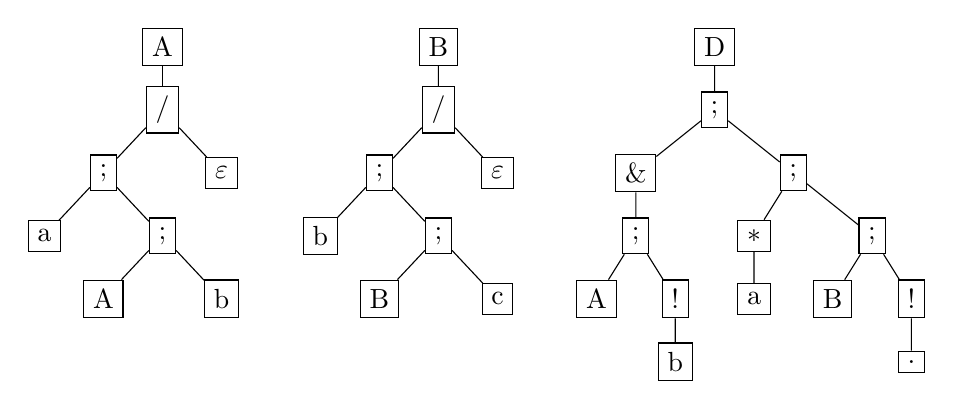
\begin{tikzpicture}%
            [level distance=8mm, every node/.style={rectangle,draw}]
            \node[wf=<7>] (A) {A}
                child {
                    node[wf=<6>] {/}
                    child {
                        node[wf=<5>] {;}
                            child { node[wf=<2>] {a} }
                            child { node[wf=<9>] {;}
                                child { node[wf=<8>] {A} }
                                child { node[wf=<2>] {b} }
                            }
                    }
                    child { node[wf=<2>] {$\PEmpty$} }
                } ;
            \node[right=30mm of A, wf=<7>] (B) {B}
                child {
                    node[wf=<6>] {/}
                    child {
                        node[wf=<5>] {;}
                            child { node[wf=<2>] {b} }
                            child { node[wf=<9>] {;}
                                child { node[wf=<8>] {B} }
                                child { node[wf=<2>] {c} }
                            }
                    }
                    child { node[wf=<2>] {$\PEmpty$} }
                } ;
            \node[right=30mm of B, wf=<12>] {D}
                child [sibling distance=20mm] {
                    node[wf=<11>] {;}
                    child {
                        node[wf=<10>] {$\&$}
                        child [sibling distance=10mm] {
                            node[wf=<9>] {;}
                            child { node[wf=<8>] {A} }
                            child {
                                node[wf=<4>] {!}
                                child { node[wf=<2>] {b} }
                            }
                        }
                    }
                    child {
                        node[wf=<10>] {;}
                        child [sibling distance=10mm] {
                            node[wf=<3>] {$*$}
                            child { node[wf=<2>] {a} }
                        }
                        child [sibling distance=20mm] {
                            node[wf=<9>] {;}
                            child [sibling distance=10mm] { node[wf=<8>] {B} }
                            child [sibling distance=10mm] {
                                node[wf=<4>] {!}
                                child { node[wf=<2>] {.} }
                            }
                        }
                    }
                } ;
        \end{tikzpicture}

        \vspace{10pt}
        \begin{overlayarea}{\textwidth}{40pt}
            \begin{itemize}
                \only<1>{\item This is the PEG for the language $a^n b^n c^n$ in tree format.}
                \only<2>{\item Empty $\PEmpty$, terminals $a, b, c$, and dot are WF.}
                \only<3>{\item Terminal $a$ is non-nullable, so $\PRepetition{a}$ is WF.}
                \only<4>{\item Not-predicates $\PNot{b}$ and $\PNot{\PDot{}}$ are WF.}
                \only<5>{\item Terminal $a$ is non-nullable, so the sequence $aAb$ is WF.
                \item The same goes for terminal $b$ and sequence $bBc$.}
                \only<6>{\item Choices $aAb/\PEmpty$ and $bBc/\PEmpty$ are WF.}
                \only<7>{\item Rules $A$ and $B$ are WF.}
                \only<8>{\item Non-terminals $A$ and $B$ are WF.}
                \only<9>{\item Sequences $Ab$, $Bc$, $A\PNot{b}$, and $B\PNot{\PDot}$ are WF.}
                \only<10>{\item And-predicate $\PAnd{(A\PNot{b})}$ is WF.
                \item Sequence $\PSequence{\PRepetition{a}}{B\PNot{\PDot}}$ is WF.}
                \only<11>{\item Sequence $\PAnd{(A\PNot{b})}\PSequence{\PRepetition{a}}{B\PNot{\PDot}}$ is WF.}
                \only<12>{\item Rule $D$ is WF.}
                \only<13>{\item Fixed point reached.
                \item All subexpressions are WF, so the grammar is WF.}
            \end{itemize}
        \end{overlayarea}
    \end{center}
\end{frame}

\begin{frame}{Not Well-Formed Grammar Example \#1}
    \begin{center}
        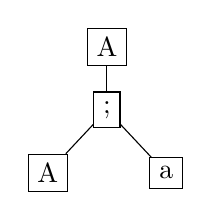
\begin{tikzpicture}%
            [level distance=8mm, every node/.style={rectangle,draw}]
            \node (A) {A}
                child {
                    node {;}
                    child { node {A} }
                    child { node[wf=<2>] {a} }
                } ;
        \end{tikzpicture}

        \vspace{10pt}
        \begin{overlayarea}{\textwidth}{50pt}
            \begin{itemize}
                \only<1>{\item This is a PEG with a single left-recursive rule $A$:
                    \begin{align*}
                        \Rule{A}{Aa}
                    \end{align*}}
                \only<2>{\item Terminal $a$ is WF.}
                \only<3>{\item Fixed point reached.
                \item Not all subexpressions are WF, so the grammar is \emph{not} WF.}
            \end{itemize}
        \end{overlayarea}
    \end{center}
\end{frame}

\begin{frame}{Not Well-Formed Grammar Example \#2}
    \begin{center}
        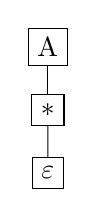
\begin{tikzpicture}%
            [level distance=8mm, every node/.style={rectangle,draw}]
            \node (A) {A}
                child {
                    node {$*$}
                    child { node[wf=<2>] {$\PEmpty$} }
                } ;
        \end{tikzpicture}

        \vspace{10pt}
        \begin{overlayarea}{\textwidth}{50pt}
            \begin{itemize}
                \only<1>{\item This is a PEG with a degenerate loop:
                    \begin{align*}
                        \Rule{A}{\PRepetition{\PEmpty}}
                    \end{align*}}
                \only<2>{\item Empty $\PEmpty$ is WF.}
                \only<3>{\item Empty $\PEmpty$ is nullable, so $\PRepetition{\PEmpty}$ is \emph{not} WF.}
                \only<4>{\item Fixed point reached.
                \item Not all subexpressions are WF, so the grammar is \emph{not} WF.}
            \end{itemize}
        \end{overlayarea}
    \end{center}
\end{frame}

\begin{frame}{\lpeg{}}
    \begin{columns}
        \begin{column}{0.7\textwidth}
            \begin{itemize}
                \item An implementation of PEGs for Lua
                \item Developed by \cite{ierusalimschy_text_2009}
                \item Features...
                \begin{itemize}
                    \item patterns as \emph{first-class citizens}
                    \item a specialized virtual machine
                    \item several interesting algorithms
                \end{itemize}
            \end{itemize}
        \end{column}
        \begin{column}{0.3\textwidth}
            \begin{figure}
                \centering
                
\includegraphics[width=0.8\textwidth]{lpeg.pdf}
            \end{figure}
        \end{column}
    \end{columns}
\end{frame}

\begin{frame}{Key Algorithms From \lpeg{}}
    \begin{itemize}
        \item Well-Formedness Check
        \item First-set Computation
    \end{itemize}
\end{frame}

\begin{frame}{\lpeg{}'s Well-Formedness Check}
    \begin{itemize}
        \item Ensures that patterns are complete
        \item Implemented in~C using simple data structures
        \item Different from the original algorithm by \citeauthor{ford_parsing_2004}
        \begin{itemize}
            \item Checks for left-recursive rules
            \item Then, checks for degenerate loops
            \item Not based on fixed-point interation
            \item Does not require complex data structures
        \end{itemize}
    \end{itemize}
\end{frame}

\begin{frame}{Left-Recursive Rules}
    \begin{itemize}
        \item Direct
        \begin{align*}
            \Rule{A}{\PChoice{\PSequence{A}{a}}{a}}
        \end{align*}
        \item Mutual
        \begin{align*}
            \begin{cases}
               \Rule{A}{\PChoice{\PSequence{B}{a}}{a}} \\
               \Rule{B}{\PChoice{\PSequence{A}{b}}{b}}
            \end{cases}
        \end{align*}
    \end{itemize}
\end{frame}

\begin{frame}{Degenerate Loops}
    \begin{align*}
        & \FordMatch{G}{e}{s}{s} \\
        & \implies \\
        & \nexists res,\ \FordMatch{G}{\PRepetition{e}}{s}{res} \\
        & \implies \\
        & \text{$G \vdash \PRepetition{e}$ is incomplete}
    \end{align*}
    \begin{itemize}
        \item Examples:
        \begin{itemize}
            \item $\PRepetition{\PEmpty}$
            \item $\PRepetition{(\POptional{e})}$
            \item $\PRepetition{(\PNot{e})}$
            \item $\PRepetition{(\PAnd{e})}$
        \end{itemize}
    \end{itemize}
\end{frame}

\begin{frame}{Well-formed Grammar Example}
    \begin{center}
        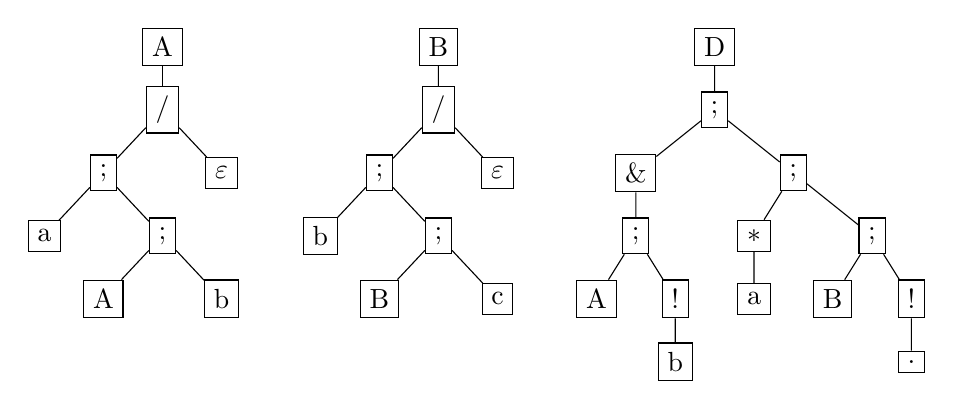
\begin{tikzpicture}%
            [level distance=8mm, every node/.style={rectangle,draw}]
            \node[wf=<6>] (A) {A}
                child {
                    node[wf=<5>] {/}
                    child {
                        node[wf=<3>] {;}
                            child { node[wf=<2>] {a} }
                            child { node {;}
                                child { node {A} }
                                child { node {b} }
                            }
                    }
                    child { node[wf=<4>] {$\PEmpty$} }
                } ;
            \node[right=30mm of A, wf=<7>] (B) {B}
                child {
                    node[wf=<7>] {/}
                    child {
                        node[wf=<7>] {;}
                            child { node[wf=<7>] {b} }
                            child { node {;}
                                child { node {B} }
                                child { node {c} }
                            }
                    }
                    child { node[wf=<7>] {$\PEmpty$} }
                } ;
            \node[right=30mm of B, wf=<21>] {D}
                child [sibling distance=20mm] {
                    node[wf=<20>] {;}
                    child {
                        node[wf=<12>] {$\&$}
                        child [sibling distance=10mm] {
                            node[wf=<11>] {;}
                            child { node[wf=<8>] {A} }
                            child {
                                node[wf=<10>] {!}
                                child { node[wf=<9>] {b} }
                            }
                        }
                    }
                    child {
                        node[wf=<19>] {;}
                        child [sibling distance=10mm] {
                            node[wf=<14>] {$*$}
                            child { node[wf=<13>] {a} }
                        }
                        child [sibling distance=20mm] {
                            node[wf=<18>] {;}
                            child [sibling distance=10mm] { node[wf=<15>] {B} }
                            child [sibling distance=10mm] {
                                node[wf=<17>] {!}
                                child { node[wf=<16>] {.} }
                            }
                        }
                    }
                } ;
        \end{tikzpicture}

        \vspace{10pt}
        \begin{overlayarea}{\textwidth}{40pt}
            \begin{itemize}
                \only<1>{\item The example PEG for the language $a^n b^n c^n$ in tree form.}
                \only<2>{\item Terminal $a$ is non-nullable.}
                \only<3>{\item Sequence $aAb$ is non-nullable.}
                \only<4>{\item Empty $\PEmpty$ is nullable.}
                \only<5>{\item Choice $aAb/\PEmpty$ is nullable.}
                \only<6>{\item Rule $A$ is nullable.}
                \only<7>{\item Rule $B$ is also nullable, by symmetry.}
                \only<8>{\item Non-terminal $A$ is nullable.}
                \only<9>{\item Terminal $b$ is non-nullable.}
                \only<10>{\item Not-predicate $\PNot{b}$ is nullable.}
                \only<11>{\item Sequence $A\PNot{b}$ is nullable.}
                \only<12>{\item And-predicate $\PAnd{(A\PNot{b})}$ is nullable.}
                \only<13>{\item Terminal $a$ is non-nullable.}
                \only<14>{\item Repetition $\PRepetition{a}$ is nullable.}
                \only<15>{\item Non-terminal $B$ is nullable.}
                \only<16>{\item Dot is non-nullable.}
                \only<17>{\item Not-predicate $\PNot{\PDot}$ is nullable.}
                \only<18>{\item Sequence $B\PNot{\PDot}$ is nullable.}
                \only<19>{\item Sequence $\PSequence{\PRepetition{a}}{B\PNot{\PDot}}$ is nullable.}
                \only<20>{\item Sequence $\PAnd{(A\PNot{b})}\PSequence{\PRepetition{a}}{B\PNot{\PDot}}$ is nullable.}
                \only<21>{\item Rule $D$ is nullable.}
                \only<22>{\item No left-recursive rules!}
            \end{itemize}
        \end{overlayarea}
    \end{center}
\end{frame}

\begin{frame}{Well-formed Grammar Example}
    \begin{center}
        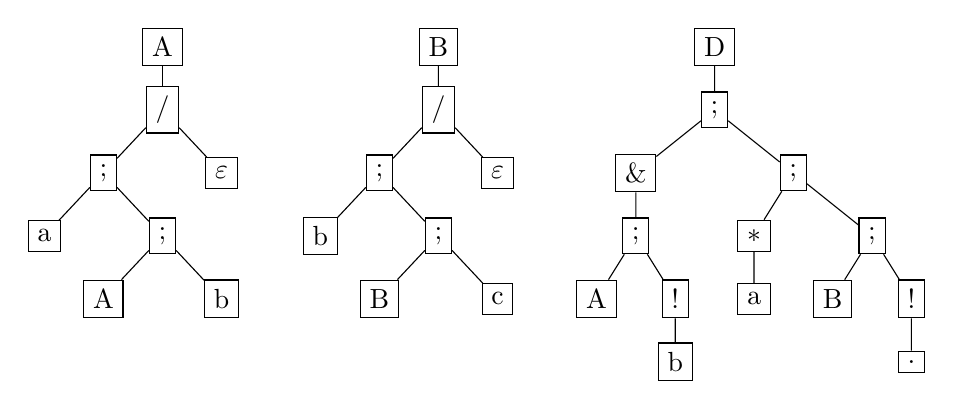
\begin{tikzpicture}%
            [level distance=8mm, every node/.style={rectangle,draw}]
            \node[wf=<9>] (A) {A}
                child {
                    node[wf=<8>] {/}
                    child {
                        node[wf=<6>] {;}
                            child { node[wf=<2>] {a} }
                            child { node[wf=<5>] {;}
                                child { node[wf=<3>] {A} }
                                child { node[wf=<4>] {b} }
                            }
                    }
                    child { node[wf=<7>] {$\PEmpty$} }
                } ;
            \node[right=30mm of A, wf=<10>] (B) {B}
                child {
                    node[wf=<10>] {/}
                    child {
                        node[wf=<10>] {;}
                            child { node[wf=<10>] {b} }
                            child { node[wf=<10>] {;}
                                child { node[wf=<10>] {B} }
                                child { node[wf=<10>] {c} }
                            }
                    }
                    child { node[wf=<10>] {$\PEmpty$} }
                } ;
            \node[right=30mm of B, wf=<24>] {D}
                child [sibling distance=20mm] {
                    node[wf=<23>] {;}
                    child {
                        node[wf=<15>] {$\&$}
                        child [sibling distance=10mm] {
                            node[wf=<14>] {;}
                            child { node[wf=<11>] {A} }
                            child {
                                node[wf=<13>] {!}
                                child { node[wf=<12>] {b} }
                            }
                        }
                    }
                    child {
                        node[wf=<22>] {;}
                        child [sibling distance=10mm] {
                            node[wf=<17>] {$*$}
                            child { node[wf=<16>] {a} }
                        }
                        child [sibling distance=20mm] {
                            node[wf=<21>] {;}
                            child [sibling distance=10mm] { node[wf=<18>] {B} }
                            child [sibling distance=10mm] {
                                node[wf=<20>] {!}
                                child { node[wf=<19>] {.} }
                            }
                        }
                    }
                } ;
        \end{tikzpicture}

        \vspace{10pt}
        \begin{overlayarea}{\textwidth}{40pt}
            \begin{itemize}
                \only<1>{\item Now, let us look for degenerate loops.}
                \only<2>{\item Terminal $a$ is OK.}
                \only<3>{\item Non-terminal $A$ is assumed to be OK.}
                \only<4>{\item Terminal $b$ is OK.}
                \only<5>{\item Sequence $Ab$ is OK.}
                \only<6>{\item Sequence $aAb$ is OK.}
                \only<7>{\item Empty $\PEmpty$ is OK.}
                \only<8>{\item Choice $aAb/\PEmpty$ is OK.}
                \only<9>{\item Rule $A$ is OK.}
                \only<10>{\item Rule $B$ is also OK, by symmetry.}
                \only<11>{\item Non-terminal $A$ is assumed to be OK.}
                \only<12>{\item Terminal $b$ is OK.}
                \only<13>{\item Not-predicate $\PNot{b}$ is OK.}
                \only<14>{\item Sequence $A\PNot{b}$ is OK.}
                \only<15>{\item And-predicate $\PAnd{(A\PNot{b})}$ is OK.}
                \only<16>{\item Terminal $a$ is OK.}
                \only<17>{\item Terminal $a$ is non-nullable, so repetition $\PRepetition{a}$ is OK.}
                \only<18>{\item Non-terminal $B$ is assumed to be OK.}
                \only<19>{\item Dot is OK.}
                \only<20>{\item Not-predicate $\PNot{\PDot}$ is OK.}
                \only<21>{\item Sequence $B\PNot{\PDot}$ is OK.}
                \only<22>{\item Sequence $\PSequence{\PRepetition{a}}{B\PNot{\PDot}}$ is OK.}
                \only<23>{\item Sequence $\PAnd{(A\PNot{b})}\PSequence{\PRepetition{a}}{B\PNot{\PDot}}$ is OK.}
                \only<24>{\item Rule $D$ is OK.}
                \only<25>{\item No denegerate loops!}
            \end{itemize}
        \end{overlayarea}
    \end{center}
\end{frame}

\begin{frame}{Not Well-Formed Grammar Example \#1}
    \begin{center}
        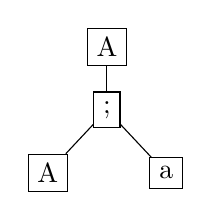
\begin{tikzpicture}%
            [level distance=8mm, every node/.style={rectangle,draw}]
            \node[visit={<2,5,8>}, ill=<9>] (A) {A}
                child {
                    node[visit={<3,6>}, ill=<11>] {;}
                    child { node[visit={<4,7>}, ill=<10>] {A} }
                    child { node {a} }
                } ;
        \end{tikzpicture}

        \vspace{10pt}
        \begin{overlayarea}{\textwidth}{50pt}
            \begin{itemize}
                \only<1>{\item This is the PEG $\{ \Rule{A}{Aa} \}$.}
                \only<2>{\item Visiting rule $A$... \item \# Non-terminals visited: 0}
                \only<3>{\item Visiting sequence $Aa$... \item \# Non-terminals visited: 0}
                \only<4>{\item Visiting non-terminal $A$... \item \# Non-terminals visited: 0}
                \only<5>{\item Visiting rule $A$... \item \# Non-terminals visited: 1}
                \only<6>{\item Visiting sequence $Aa$... \item \# Non-terminals visited: 1}
                \only<7>{\item Visiting non-terminal $A$... \item \# Non-terminals visited: 1}
                \only<8>{\item Visiting rule $A$... \item \# Non-terminals visited: 2}
                \only<9>{\item Visited more rules than the number of grammar rules. \item Rule $A$ is left-recursive!}
                \only<10>{\item Non-terminal $A$ leads to left recursion.}
                \only<11>{\item Sequence $Aa$ leads to left recursion.}
                \only<12>{\item Grammar contains a left-recursive rule.}
            \end{itemize}
        \end{overlayarea}
    \end{center}
\end{frame}

\begin{frame}{Not Well-Formed Grammar Example \#2}
    \begin{center}
        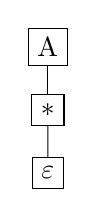
\begin{tikzpicture}%
            [level distance=8mm, every node/.style={rectangle,draw}]
            \node[visit={<2>}, wf=<7>] (A) {A}
                child {
                    node[visit={<3>}, wf=<6>] {$*$}
                    child { node[visit={<4>}, wf=<5>] {$\PEmpty$} }
                } ;
        \end{tikzpicture}

        \vspace{10pt}
        \begin{overlayarea}{\textwidth}{50pt}
            \begin{itemize}
                \only<1>{\item This is the PEG $\{ \Rule{A}{\PRepetition{\PEmpty}} \}$.}
                \only<2>{\item Visiting rule $A$...}
                \only<3>{\item Visiting repetition $\PRepetition{\PEmpty}$...}
                \only<4>{\item Visiting empty $\PEmpty$...}
                \only<5>{\item Empty $\PEmpty$ is nullable.}
                \only<6>{\item Repetition $\PRepetition{\PEmpty}$ is nullable.}
                \only<7>{\item Rule $A$ is nullable.}
                \only<8>{\item No left-recursive rule.}
            \end{itemize}
        \end{overlayarea}
    \end{center}
\end{frame}

\begin{frame}{Not Well-Formed Grammar Example \#2}
    \begin{center}
        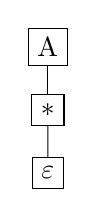
\begin{tikzpicture}%
            [level distance=8mm, every node/.style={rectangle,draw}]
            \node[visit=<2>, ill=<7>] (A) {A}
                child {
                    node[visit=<3>, ill=<6>] {$*$}
                    child { node[visit=<4>, wf=<5>] {$\PEmpty$} }
                } ;
        \end{tikzpicture}

        \vspace{10pt}
        \begin{overlayarea}{\textwidth}{50pt}
            \begin{itemize}
                \only<1>{\item Now, let us look for degenerate loops.}
                \only<2>{\item Visiting rule $A$...}
                \only<3>{\item Visiting repetition $\PRepetition{\PEmpty}$...}
                \only<4>{\item Visiting empty $\PEmpty$...}
                \only<5>{\item Empty $\PEmpty$ has no degenerate loops.}
                \only<6>{\item Empty $\PEmpty$ is nullable, so repetition $\PRepetition{\PEmpty}$ is degenerate.}
                \only<7>{\item Rule $A$ has a degenerate loop.}
                \only<8>{\item Grammar has a degenerate loop.}
            \end{itemize}
        \end{overlayarea}
    \end{center}
\end{frame}

\begin{frame}{Properties of \lpeg{}'s Well-Formedness Check}
    \begin{itemize}
        \item Termination
        \item Correctness
    \end{itemize}
\end{frame}

\begin{frame}{First-Set}
    \begin{align*}
        & \text{$a \notin$ first-set of $G \vdash e$} \\
        & \implies \\
        & \forall s,\ \FordMatch{G}{e}{a::s}{\bot}
    \end{align*}
    \begin{itemize}
        \item ``Which first characters make a pattern fail?''
        \item Concept originally from $LL(1)$ parsers
    \end{itemize}
\end{frame}

\begin{frame}{Emptiness}
    \begin{align*}
        & \text{$G \vdash e$ is not empty} \\
        & \implies \\
        & \FordMatch{G}{e}{\varepsilon}{\bot}
    \end{align*}
    \begin{itemize}
        \item ``Does the pattern fail the empty string?''
        \item Sometimes denoted as $\varepsilon \in first(e)$ in $LL(1)$
    \end{itemize}
\end{frame}

\begin{frame}{First-Set and Emptiness in \lpeg{}}
    \begin{itemize}
        \item Both values are computed by the same function
        \item \lpeg{} uses them to optimize certain patterns
    \end{itemize}
\end{frame}

\begin{frame}{Properties of First-Set Computation}
    \begin{itemize}
        \item It terminates for any well-formed grammar and expression
        \item It correctly identifies first characters that make a pattern fail
        \item It correctly identifies patterns that fail the empty string
    \end{itemize}
\end{frame}

% \newcommand{\SlidesFirstA}[2]{\firstname{}(#1,#2)}
%
% \begin{frame}{First-Set Property}
%     \begin{align*}
%         & c \notin \SlidesFirstA{G}{p} \\
%         & \implies \\
%         & \forall s,\ \FordMatch{G}{p}{c::s}{\bot}
%     \end{align*}
% \end{frame}
%
% \begin{frame}{First-Set of some Patterns}
%     \begin{itemize}
%         \item $\SlidesFirstA{G}{\PEmpty} = \Sigma$
%         \item $\SlidesFirstA{G}{\PRepetition{p}} = \Sigma$
%         \item $\SlidesFirstA{G}{\PSet{cs}} = \Set{cs}$
%     \end{itemize}
% \end{frame}
%
% \begin{frame}{First-Set of Sequences}
%     \begin{align*}
%         \SlidesFirstA{G}{\PSequence{p_1}{p_2}} &=
%         \begin{cases}
%             \SlidesFirstA{G}{p_1} & \text{if $p_1$ is non-nullable} \\
%             \dots? & \text{if $p_1$ is nullable}
%         \end{cases}
%     \end{align*}
% \end{frame}
%
% \begin{frame}{First-Set of Sequences of Nullable Patterns}
%     \begin{itemize}
%         \item $\SlidesFirstA{G}{\PSequence{\PEmpty}{\PSet{cs_2}}} = \Set{cs_2}$
%         \item $\SlidesFirstA{G}{\PSequence{\PRepetition{\PSet{cs_1}}}{\PSet{cs_2}}} = \SetUnion{\Set{cs_1}}{\Set{cs_2}}$
%     \end{itemize}
% \end{frame}
%
% \newcommand{\SlidesFirstB}[3]{\firstname{}(#1, #2, #3)}
%
% \begin{frame}{Follow-Set Parameter}
%     \begin{itemize}
%         \item $\SlidesFirstB{G}{\PEmpty}{follow} = follow$
%         \item $\SlidesFirstB{G}{\PRepetition{p}}{follow} = \SlidesFirstB{G}{p}{follow} \cup follow$
%         \item $\SlidesFirstB{G}{\PNot{p}}{follow} = follow$
%         \item $\SlidesFirstB{G}{\PAnd{p}}{follow} = \SlidesFirstB{G}{p}{\Sigma} \cap follow$
%     \end{itemize}
% \end{frame}
%
% \begin{frame}{Follow-Set Independence of Non-Nullable Patterns}
%     \begin{align*}
%         & \text{$G \vdash p$ is non-nullable} \\
%         & \implies \\
%         & \forall follow_1,\ \forall follow_2, \\
%         & \SlidesFirstB{G}{p}{follow_1} = \SlidesFirstB{G}{p}{follow_2}
%     \end{align*}
% \end{frame}
%
% %         \begin{align*}
% %             c \notin First(G, e) \implies \forall s, \FordMatch{G}{e}{c::s}{\bot}
% %         \end{align*}
%
% \begin{frame}{First-Set Function Signature}
%     \begin{itemize}
%         \item Takes a grammar $G$, a pattern $p$, a follow-set $follow$
%         \item Returns the first-set and the emptiness value of $G \vdash p$
%         \item Concept imported from $LL(1)$ parsers, and adapted to PEGs
%         \item Set of first characters that can be accepted by a pattern
%     \end{itemize}
% \end{frame}
%
% \begin{frame}{Properties of \lpeg{}'s First-Set Computation}
%     \begin{itemize}
%         \item Terminates for any well-formed PEG
%         \item Indicates first characters that make a pattern fail:
%         \begin{align*}
%             c \notin first(G, e) \implies \forall s, \FordMatch{G}{e}{c::s}{\bot}
%         \end{align*}
%         \item Also checks whether a pattern fails the empty string:
%         \begin{align*}
%             \neg empty(G, e) \implies \FordMatch{G}{e}{\EmptyString}{\bot}
%         \end{align*}
%     \end{itemize}
% \end{frame}
%
% % \newcommand{\ifthenelsepat}[3]{\PChoice{\PSequence{\PAnd{#1}}{#2}}{\PSequence{\PNot{#1}}{#3}}}
%
% \begin{frame}{Follow-Set}
%     \begin{itemize}
%         \item
%     \end{itemize}
% \end{frame}
%
% \begin{frame}{Application of First-Set in \lpeg{}}
%     \begin{itemize}
%         \item Assume $G \vdash \PChoice{e_1}{e_2}$ is well-formed.
% % and $s'$ either is empty or starts with $x \in follow$, \\
% % and $\firstcomp{g}{p_1}{\Sigma}{gas_1} = \Some (false, first_1)$, \\
% % and $\firstcomp{g}{p_2}{follow}{gas_2} = \Some (b, first_2)$, \\
% % and $\SetIntersection{first_1}{first_2} = \EmptySet{}$, \\
% % and $\Matches{g}{\PChoice{p_1}{p_2}}{s}{s'}$, \\
% % then $\Matches{g}{\ifthenelsepat{\PSet{first_1}}{p_1}{p_2}}{s}{s'}$.
%     \end{itemize}
% \end{frame}

\begin{frame}{Related Work}
    \begin{itemize}
        \item \cite{ford_parsing_2004} introduced PEGs
        \item \cite{koprowski_trx_2011} and \emph{well-formed} XPEGs in Coq
        \item \cite{ribeiro_towards_2019} and \emph{well-typed} PEGs in Agda
        \item \cite{blaudeau_verified_2020} and their verified PEG parser in PVS
    \end{itemize}
\end{frame}

\begin{frame}{Conclusion}
    \begin{itemize}
        \item We formalized two algorithms from \lpeg{}:
        \begin{itemize}
            \item the well-formedness check;
            \item and the first-set computation.
        \end{itemize}
        \item We proved their termination and correctness
        \item We identified opportunities for improvements in \lpeg{}
    \end{itemize}
\end{frame}

% Hide bibliography
\begin{frame}<beamer:0>
    \bibliographystyle{apalike}
    \bibliography{references}
\end{frame}

\end{document}
